\chapter{Implementación y Experimentos} 
\section{Experimentos} 

\begin{figure}[H]
  \begin{center}
    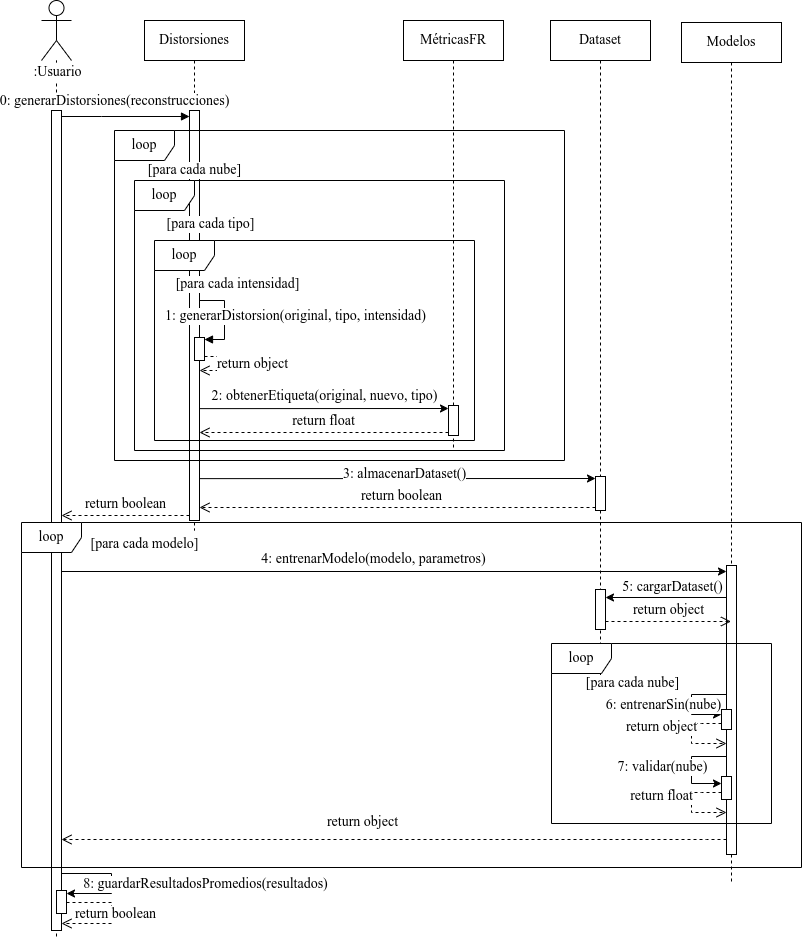
\includegraphics[width=0.90\textwidth]{imagenes/chapter5/TFGSequence}
  \end{center}
  \caption{Diagrama de secuencias del proyecto.}
  \label{fig:TFGSequence}
\end{figure}

Todo el código desarrollado se encuentra 
en el GitHub \url{https://github.com/CodeBoy-source/TFG_NRPCQA}.
En la Figura \ref{fig:TFGSequence} se observa el diagrama de secuencias 
que determina el flujo de tareas implementadas para el desarrollo de este proyecto. 
Se divide en dos grandes bloques: la generación de los datos sintéticos y 
la obtención de los resultados promedios de los modelos. A continuación 
se expone el proceso de obtención de dichos resultados y el correspondiente
análisis de cada uno de ellos. 

\subsection{Protocolo de validación experimental} 
\label{sec:Validation}

\begin{figure}[htp]
 \begin{center}
   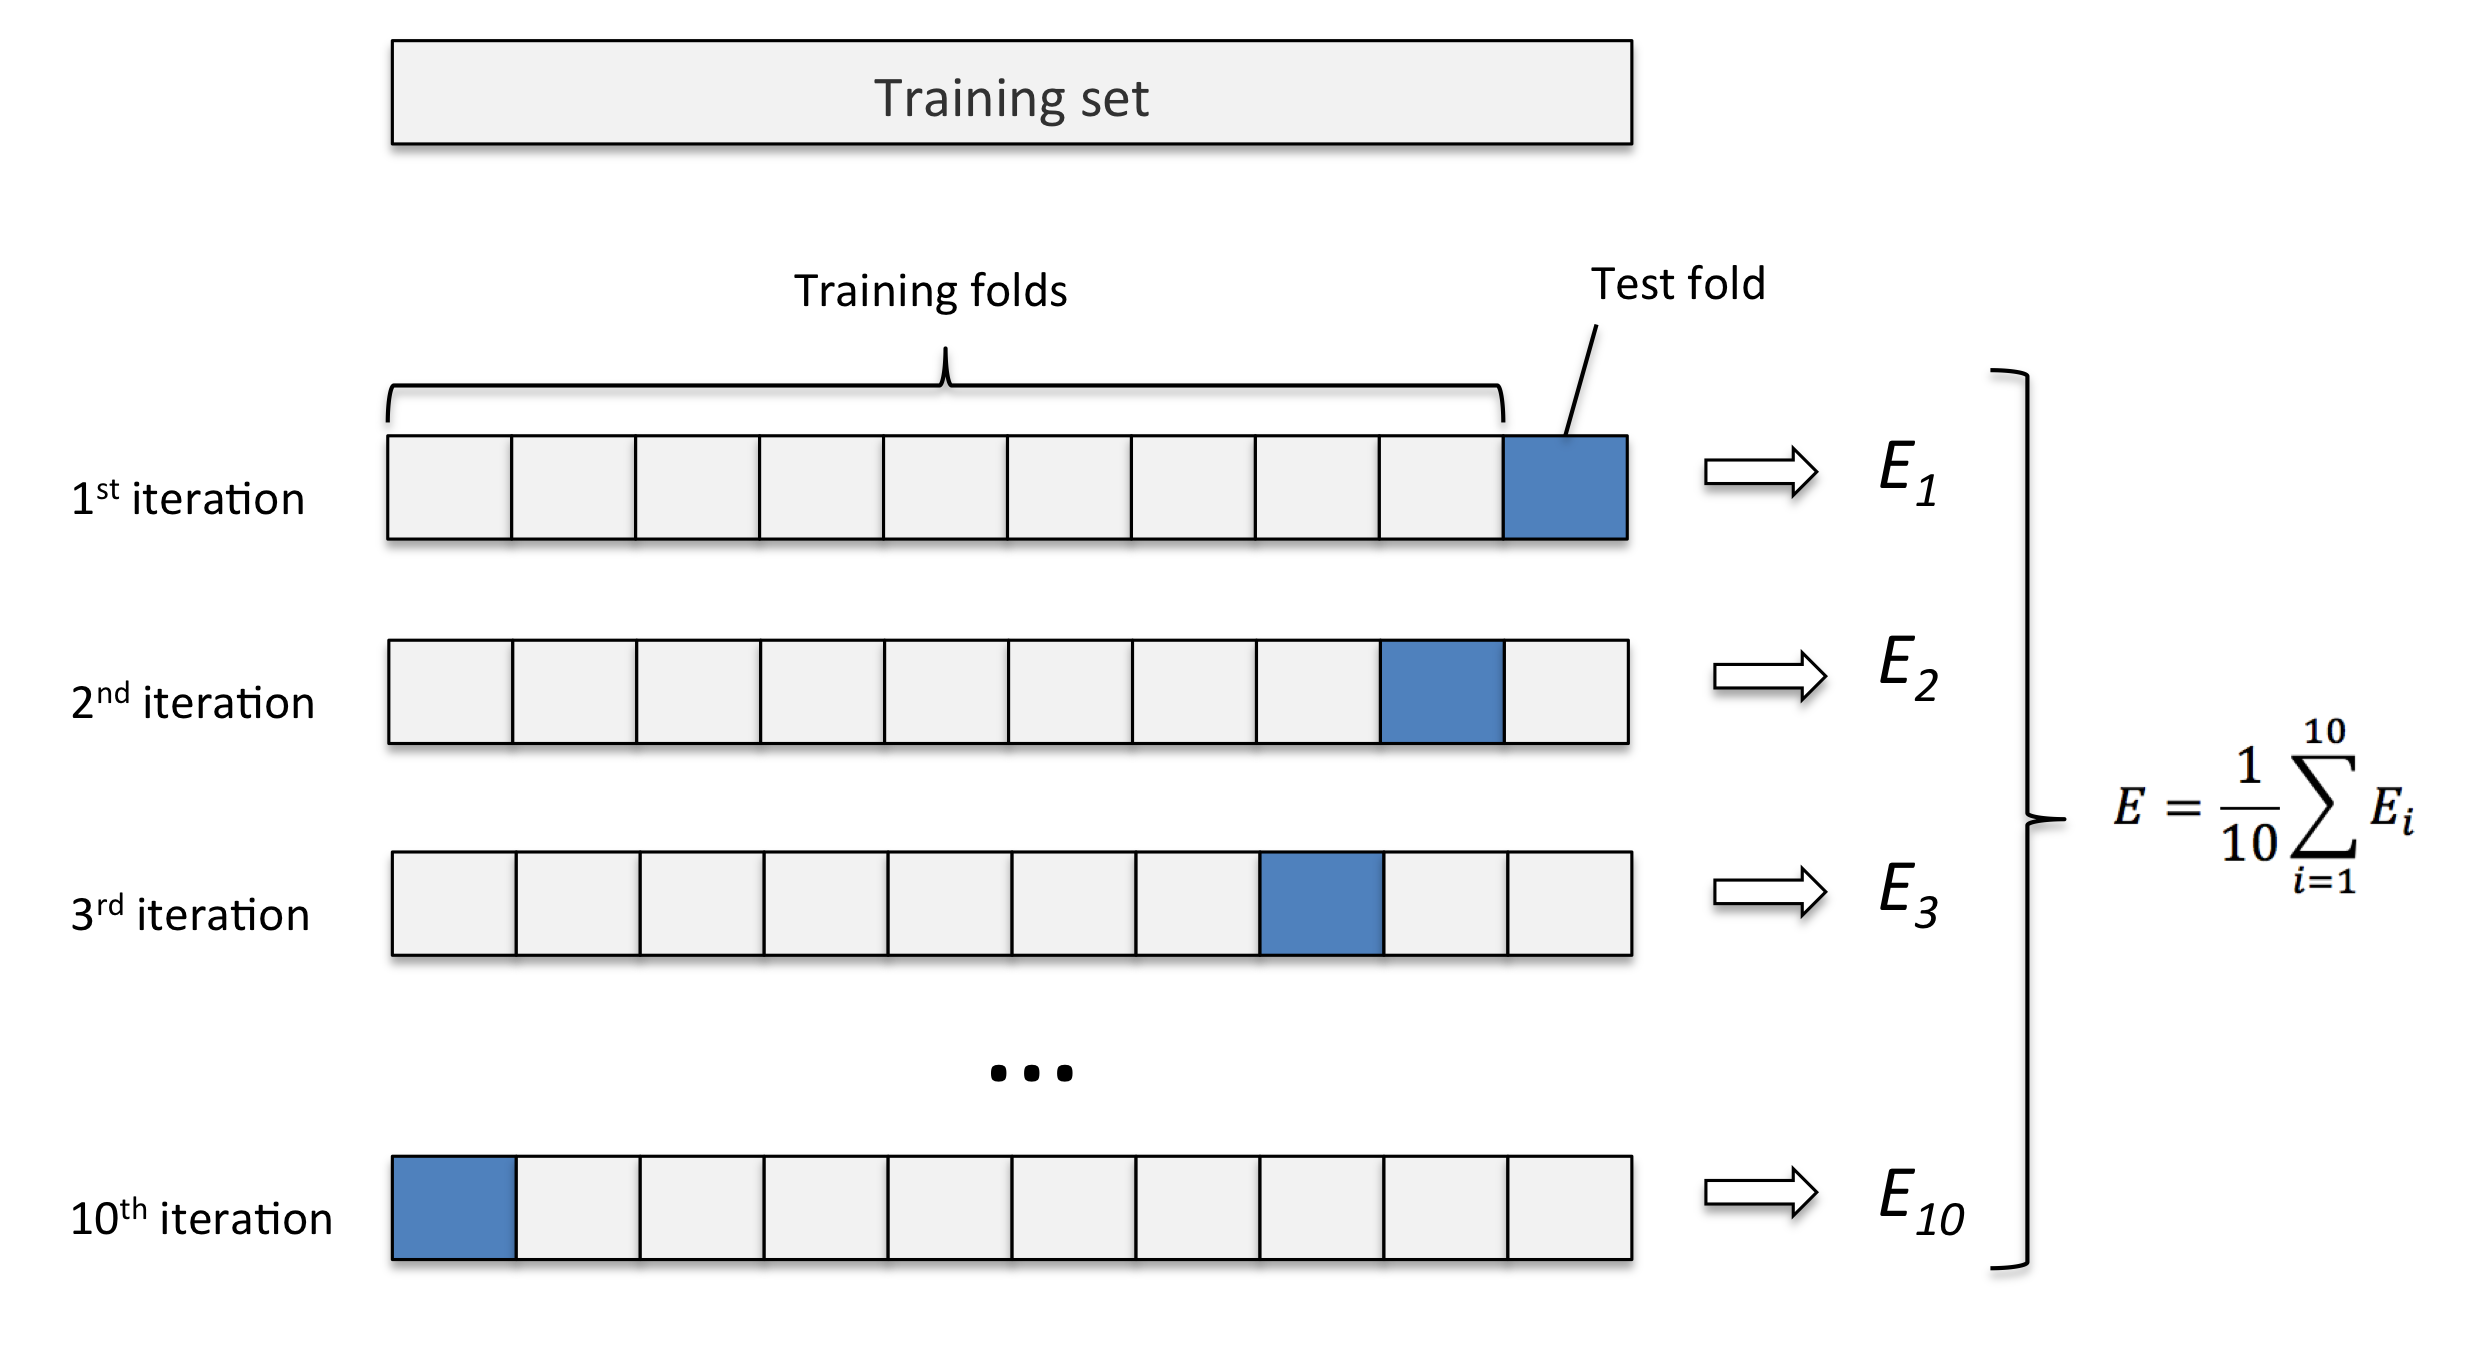
\includegraphics[width=\textwidth]{imagenes/chapter5/cross-validation}
 \end{center}
 \caption{Ejemplo de uso de K-fold para la búsqueda de hiperparámetros.}
 \label{fig:K-fold}
\end{figure}

Para la validación del modelo y la estimación de su rendimiento para las distintas 
mejoras propuestas se ha utilizado la técnica de \emph{cross-validation} ó 
validación cruzada, también conocida por \emph{K-fold}. 
Esta técnica se distingue por realizar la división del conjunto de datos 
en K partes (pliegues). A continuación el modelo se entrena y evalúa K veces, utilizando 
cada una de los pliegues como conjunto de prueba y el resto de los pliegues como 
conjunto de entrenamiento en cada iteración (véase Figura \ref{fig:K-fold}). 
Al finalizar las K iteraciones, se promedia los resultados de evaluación 
obtenidos para obtener una medida general de rendimiento. 
Es decir, un K-fold con K=1 equivale a la técnica de \emph{hold-out} 
donde se divide el conjunto de datos en el conjunto de entrenamiento y 
el conjunto de test.  

En el caso de nuestro dataset de imágenes médicas, al ser pocos ejemplos 
se ha realizado un pliegue por modelo 3D, así que por cada pliegue hay un total de 
350 ejemplos de entrenamiento y 35 ejemplos en test. 
En el caso de pre-entrenar usando LS-SJTU-PCQA~\cite{ResSCNN}, con 3640 ejemplos en total para 
nuestras distorsiones, se optó por utilizar 80\% para entrenamiento y 20\% para test. 
Para las pruebas preliminares se utilizó el conjunto SJTU con las condiciones indicadas por 
\cite{VQA-PC}, es decir, con nueve pliegues, uno por modelo para un total de 336 ejemplos para entrenamiento y 42 para test. 

Primeramente se replican los resultados obtenidos en las publicaciones originales 
de los métodos NR3DQA~\cite{NR3DQA} y VQA-PC~\cite{VQA-PC}. Para ello se utilizan
los conjuntos de datos públicos SJTU~\cite{SJTU} y WPC~\cite{WPC1,WPC2}. 
A continuación, se analizan los resultados obtenidos sobre nuestro conjunto 
de imágenes médicas y, con ello, se proponen mejoras y adaptaciones con fin 
de obtener mejores resultados. 

\subsection{Experimentos NR3DQA}
Para replicar el método de Zhang et al~\cite{NR3DQA} podemos utilizar los 
scripts en \code{NR3DQA/}. Para ello disponemos de unos cuántos scripts para la extracción de las características y visualización de las distribuciones 
como indica la publicación (ver Apéndice \ref{sec:Implementacion}). 
Utilizaremos la librería de Pyntcloud~\cite{Pyntcloud} para obtener 
la matriz de covarianza y calcular las características en base a lo definido 
en la Sección \ref{sec:NR3DQA}.
Para los conjuntos de datos SJTU y WPC, los resultados 
son similares a los obtenidos en la publicación original (véase Tabla \ref{tab:PlainNR3DQA}).
Hay que tener en cuenta que para ambos se realiza un K-fold, donde el número 
K es igual al número de nubes de puntos 

\begin{table}[htp]
  \scriptsize
  \begin{center}
    \begin{tabular}[c]{|c|c|c|c|c|}
      \hline
      \rowcolor[HTML]{FFC702}
      \textbf{Dataset} & \textbf{PLCC} & \textbf{SROCC} & \textbf{KROCC} \\ 
      \hline
      SJTU & \textbf{0.810325} & \textbf{0.777403} & \textbf{0.608302} \\ 
      \hline 
      WPC & 0.637953 & 0.634853 & 0.463578 \\
      \hline
    \end{tabular}
  \end{center}
  \caption[Resultados de prueba preliminar con SVM.]{Resultados de prueba preliminar con SVM.
  En SJTU tenemos una mejora de 7\% respecto a la publicación original que podemos asociar al ruido de la inicialización aleatoria. }
  \label{tab:PlainNR3DQA}
\end{table}

No obstante, utilizando las mismas funciones para el caso de los imágenes médicas 
y experimentando con múltiples modelos de regresión, 
vemos, en la Tabla \ref{tab:MedicalNR3DQA}, que el método no es capaz
de determinar con precisión la calidad de imágenes, ya que la correlación entre 
la predicción y el valor real es muy cercano a 0. 
Incluso utilizando el conjunto SJTU para ayudar al entrenamiento 
del SVM, no obtenemos mejoras significativas, sino que obtenemos un 0.225 de SROCC.


\begin{table}[htp]
  \scriptsize
  \begin{center}
    \hspace{-.5cm}
    \begin{tabular}[c]{|c|c|c|c|c|}
      \hline
      \rowcolor[HTML]{FFC702}
      \multicolumn{1}{|c|}{\textbf{Etiqueta Sintética}} & 
      \multicolumn{1}{|c|}{\textbf{Modelo}} & 
      \multicolumn{1}{|c|}{\textbf{Escalado}} & 
      \multicolumn{1}{|c|}{\textbf{PLCC}} &
      \multicolumn{1}{|c|}{\textbf{SROCC}} \\
      \hline
      Valor de la métrica & SVM & RobustScaler & 0.2017 & 0.1776 \\
      \hline
      Valor normalizado & KNNRegressor & RobustScaler & 0.2671 & 0.1882  \\
      \hline
      Valor en escala 0-5 & DecisionTree & StandardScaler & \textbf{0.309176} & \textbf{0.196713} \\
      \hline
    \end{tabular}
  \end{center}
  \caption[Resultados de prueba preliminar con SVM.]{Resultados de prueba preliminar con SVM. 
  Vemos los mejores modelos y normalización para las diferentes escalas de las etiquetas sintéticas. 
  Se observa que con el conjunto de imágenes médicas no hemos logrado buena correlación entre 
  los valores predichos y el valor real.}
  \label{tab:MedicalNR3DQA}
\end{table}

Algo similar ocurre cuando intentamos utilizar más características geométricas
como se indica en el trabjo de Weinmann et al~\cite{3DNSSMetrics}. Se argumenta que, en el proceso de segmentación, 
detección y clasificación de estructuras en nubes de puntos, 
las mejores métricas suelen ser: 
omnivarianza, entropía de valores singulares, la verticalidad del vecindario y 
otras. Los resultados de utilizar estas métricas adicionales, que 
se pueden observar en la Tabla \ref{tab:ImprovNR3DQA}, no son significativos.


\begin{table}[htp]
  \scriptsize
  \begin{center}
    \begin{tabular}[c]{|c|c|c|c|c|}
      \hline
      \rowcolor[HTML]{FFC702}
      \textbf{Dataset} & \textbf{PLCC} & \textbf{SROCC} & \textbf{KROCC} \\ 
      \hline
      SJTU & \textbf{0.853709} & \textbf{0.820057} & \textbf{0.649406} \\ 
      \hline 
      WPC & 0.642356 & 0.62917 & 0.455562 \\
      \hline 
      Nuestro & 0.344601 &  0.170793 & -- \\
      \hline
    \end{tabular}
  \end{center}
  \caption[Resultado de mejores sobre el método SVM]{Resultado de mejores sobre el método SVM.
   Se observa mejoras, no sustanciales, sobre los conjuntos SJTU, WPC e imágenes médicas.
   No obstante, todavía sigue por detrás de los métodos DL, como el método VQA-PC 
   que se discutirá más adelante.
  }
  \label{tab:ImprovNR3DQA}
\end{table}

En el estado del arte vimos que hay cierta inclinación al uso de modelos 
DL para intentar superar los resultados actuales y obtener una métrica más 
genérica. Se observa la dificultad del análisis de NSS a la hora de elegir que métricas 
deben extraerse para generar un buen vector características para un modelo ML 
que intenta resolver este problema. Dado el marco temporal y visto los 
resultados preliminares de la Sección \ref{sec:PreResults}, se determina 
conveniente hacer uso de modelos más complejos y permitir que la extracción 
de características sea automática. 

\subsection{Experimentos VQA-PC}
\label{sec:PreResults}
Previo a tratar con los datos médicos, se han realizado pruebas de ejecución 
para verificar el funcionamiento del modelo, validar los resultados, familiarizarse 
con el código e identificar zonas de posibles mejoras.

\subsubsection{Replicando los resultados sobre SJTU}
\label{sec:VQAPCSJTU}
Para validar el correcto funcionamiento del código y los resultados obtenidos 
en~\cite{VQA-PC}, realizamos el experimento en las mismas condiciones descrita 
por ellos en el conjunto de datos SJTU. Como ese posee 10 modelos, 
(ver Sección \ref{sec:DatosPublicos}) se realiza un 9-fold. Se han utilizado 
los mismos hiperparámetros, estructura de red convolucional y transformaciones 
de datos (véanse Tablas \ref{tab:ResNet50} y \ref{tab:HiperSJTU}). 

\begin{table}[htp]
  \scriptsize
  \begin{center}
    \begin{tabular}[c]{|c|c|}
      \hline
      \rowcolor[HTML]{FFC702}
      \textbf{Hiperparámetro} & \textbf{Valor} \\ 
      \hline 
      Tasa de aprendizaje &  0.0004 \\ 
      \hline 
      Tamaño de batches & 32 \\ 
      \hline 
      Tasa de decadencia & 0.9 \\ 
      \hline 
      Frecuencia de decadencia & 10 \\ 
      \hline 
      Épocas & 30 \\ 
      \hline 
      K-fold & 9 \\ 
      \hline 
    \end{tabular}
  \end{center}
  \caption[Hiperparámetros empleados en la experimentación preliminar.]{
    Hiperparámetros empleados en la experimentación preliminar~\cite{VQA-PC}.
  }
  \label{tab:HiperSJTU}
\end{table}

Para el conjunto de entrenamiento se recorta una zona aleatoria de la imagen con 
tamaño 224x224, a continuación se normaliza los colores conforme al siguiente 
vector de medias $\mu = \left[ 0.485, 0.456, 0.406 \right]$ y de desviación típica
$\sigma = \left[ 0.229, 0.224, 0.225 \right]$. Valores con los cuales se 
normalizaron las imágenes con las que entrenó ResNet~\cite{ResNet}.
Para el conjunto de test, se utiliza la misma normalización de colores, pero 
en vez de recortar una zona aleatoria de la imagen se recorta la parte central. 

\bgroup
\begin{table}[htp]
  \scriptsize
  \begin{center}
    % \[\setcellgapes{5pt}\makegapedcells % <--- for vertical space around cells contents
    \begin{tabular}[b]{|c|c|c|}
      \hline
      \rowcolor[HTML]{FFC702}
      \multicolumn{1}{|c|}{\textbf{Capa}} & \multicolumn{1}{c|}{\textbf{Salida}}  &
      \multicolumn{1}{c|}{\textbf{Estructura}} \\
      \hline
      Bloque inicial & $112\times112$ & $7\times7,\; 64$, stride 2 \\ 
      \hline 
      \multirow{2}{*}{Bloque convolucional 1} & \multirow{2}{*}{$56\times56$} & $3\times3$ max pool, stride 2 \\ 
      \cline{3-3}
                                              & & $\begin{bmatrix}1\times1,\; 64 \\ 3\times3,\; 64 \\ 1\times1,\; 256 \end{bmatrix}\times 3$ \\ 
      \hline
      Bloque convolucional 2 & $28\times28$ & $\begin{bmatrix}1\times1,\; 128 \\ 3\times3,\; 128 \\ 1\times1,\; 512 \end{bmatrix}  \times 3 $\\ 
      \hline
      Bloque convolucional 3 & $14\times14$ & $\begin{bmatrix}1\times1,\; 256 \\ 3\times3,\; 256 \\ 1\times1,\; 1024 \end{bmatrix} \times 3$ \\ 
      \hline
      Bloque convolucional 4 & $7\times7$   & $\begin{bmatrix}1\times1,\; 512 \\ 3\times3,\; 512 \\ 1\times1,\; 2048 \end{bmatrix}  \times 3 $\\ 
      \hline
      Bloque convolucional 5 & $1\times1$   & average pool, 1000-d fc, softmax\\ 
      \hline
      \multicolumn{2}{|r|}{\cellcolor[HTML]{FFC702}\textbf{Total de parámetros}} & \textbf{23.803.969}\\
      \hline 
      \end{tabular}
    % \]
  \end{center}
  \caption{Descripción de la arquitectura ResNet50.}
  \label{tab:ResNet50}
\end{table}
\egroup

Tras pasada las 9 iteraciones, el resultado promedio es similar al estimado 
por el artículo original y, como se puede observar en la Figura \ref{fig:PreTestCurves},
el modelo parece estar aprendiendo. Los resultados se reflejan
en la Tabla \ref{tab:PreTestResults}. 
Como vemos el error de validación tiende a bajar, aunque con cierta variabilidad 
entre épocas en contra del error de entrenamiento que es más estable. . 

Se debe tener en cuenta que, aunque el error cuadrático medio (MSE, por sus siglas en inglés) pueda parecer 
sustancialmente grande, nuestro criterio de elección sería la correlación 
entre las métricas. Es decir, no necesitamos estimar los valores de distorsión 
en la misma escala que las etiquetas. Apenas necesitamos ser capaces de comparar 
de forma ordenada las imágenes de menor a mayor calidad. En otras palabras, 
si la función a determinar es $f(x) = x$, tener $f(x) = 100x$ sería equivalente.
Por ello, de aquí en adelante utilizaremos la métrica SROCC.
Cabe observar que los valores se acercan a los resultados obtenidos en la publicación original, 
utilizando el criterio del promedio del mejor resultado de cada pliegue de validación. 

\begin{table}[htp]
  \scriptsize
  \begin{center}
    \begin{tabular}[c]{|c|c|c|}
      \hline
      \rowcolor[HTML]{FFC702}
      \textbf{Kfold} & \textbf{MSE} & \textbf{SROCC} \\ 
      \hline 
      0 & 13.9222 & 0.8995 \\
      \hline 
      1 & 418120.5625 & 0.8547 \\ 
      \hline 
      2 & 10.9271 & 0.9081 \\
      \hline 
      3 & 19.8226 & 0.9295 \\ 
      \hline 
      4 & 443.6077 & 0.8700 \\ 
      \hline 
      5 & 28.3165 & 0.9544 \\ 
      \hline 
      6 & 292.239 & 0.7675 \\ 
      \hline 
      7 & 329.0685 & 0.8833 \\ 
      \hline 
      8 & 357.0455 & 0.8647 \\ 
      \hline
      \textbf{\cellcolor[HTML]{FFC702}Promedio} & \textbf{46623.94} & \textbf{0.8813} \\ 
      \hline
    \end{tabular}
  \end{center}
  \caption[Resultados de experimento preliminar.]{
    Resultados de experimento preliminar. 
    Se enseña el MSE del modelo sin utilizar la regresión logística para normalizar las distancias.
  }
  \label{tab:PreTestResults}
\end{table}

\begin{figure}[htp]
  \begin{subfigure}[b]{0.49\textwidth}
  \centering
    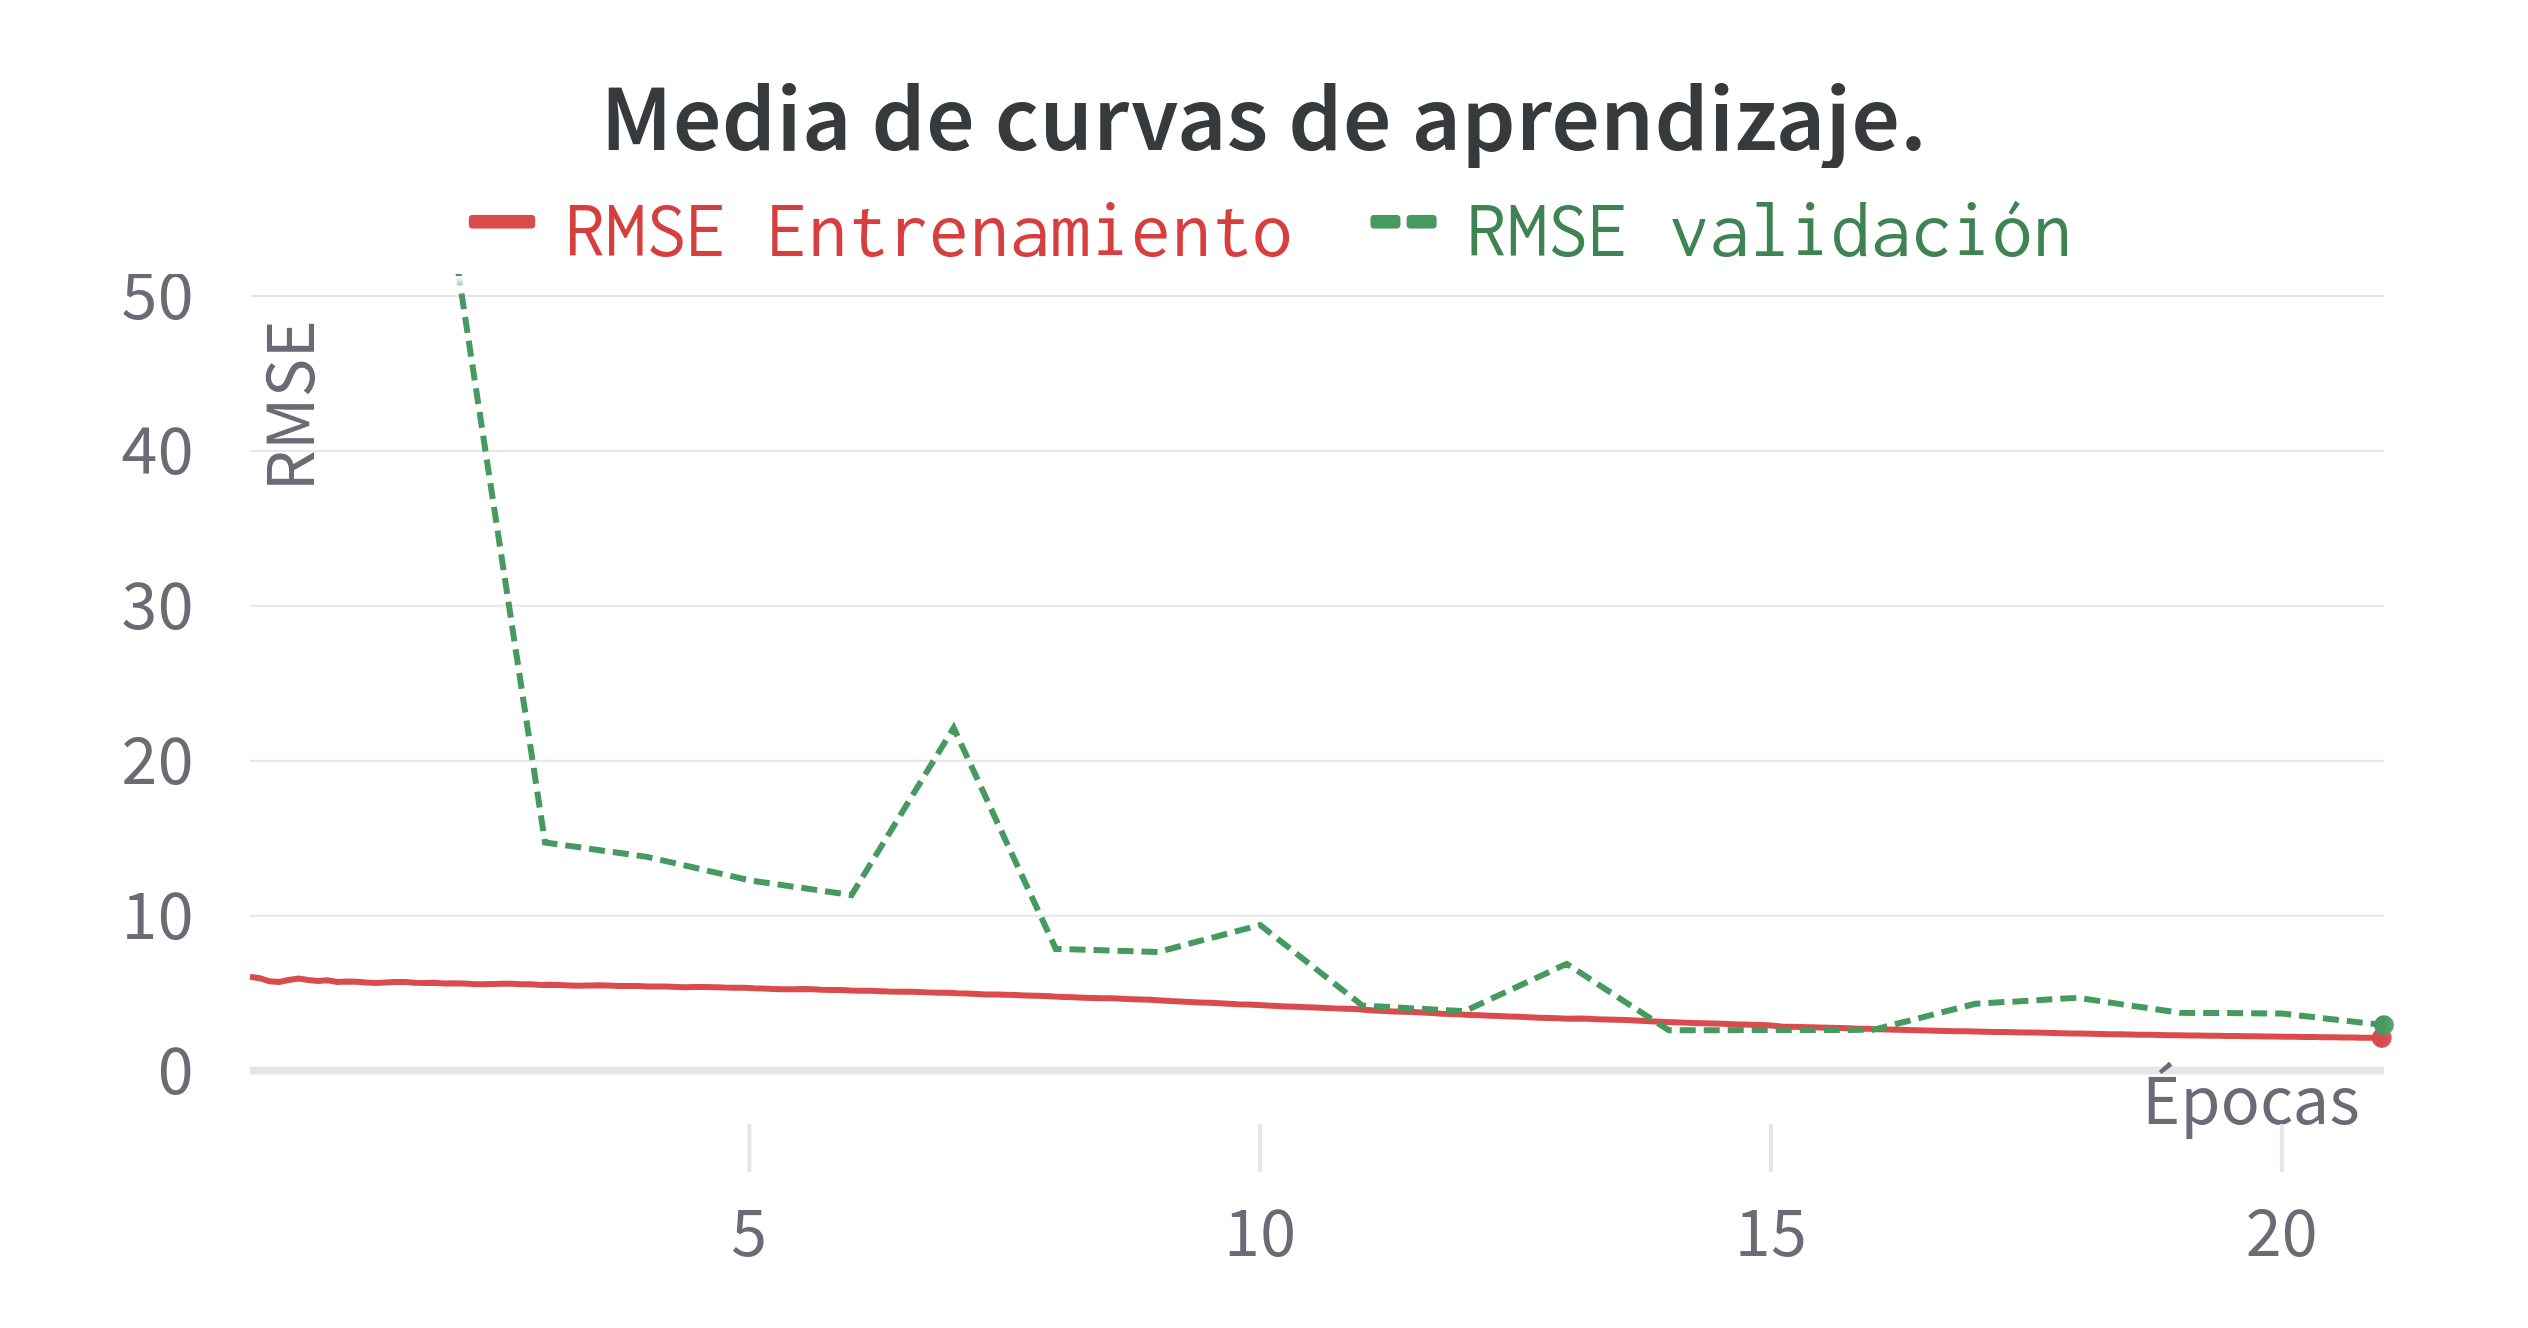
\includegraphics[width=\textwidth]{imagenes/chapter5/PreTestCurves.png}
  \end{subfigure}
  \begin{subfigure}[b]{0.49\textwidth}
  \centering
    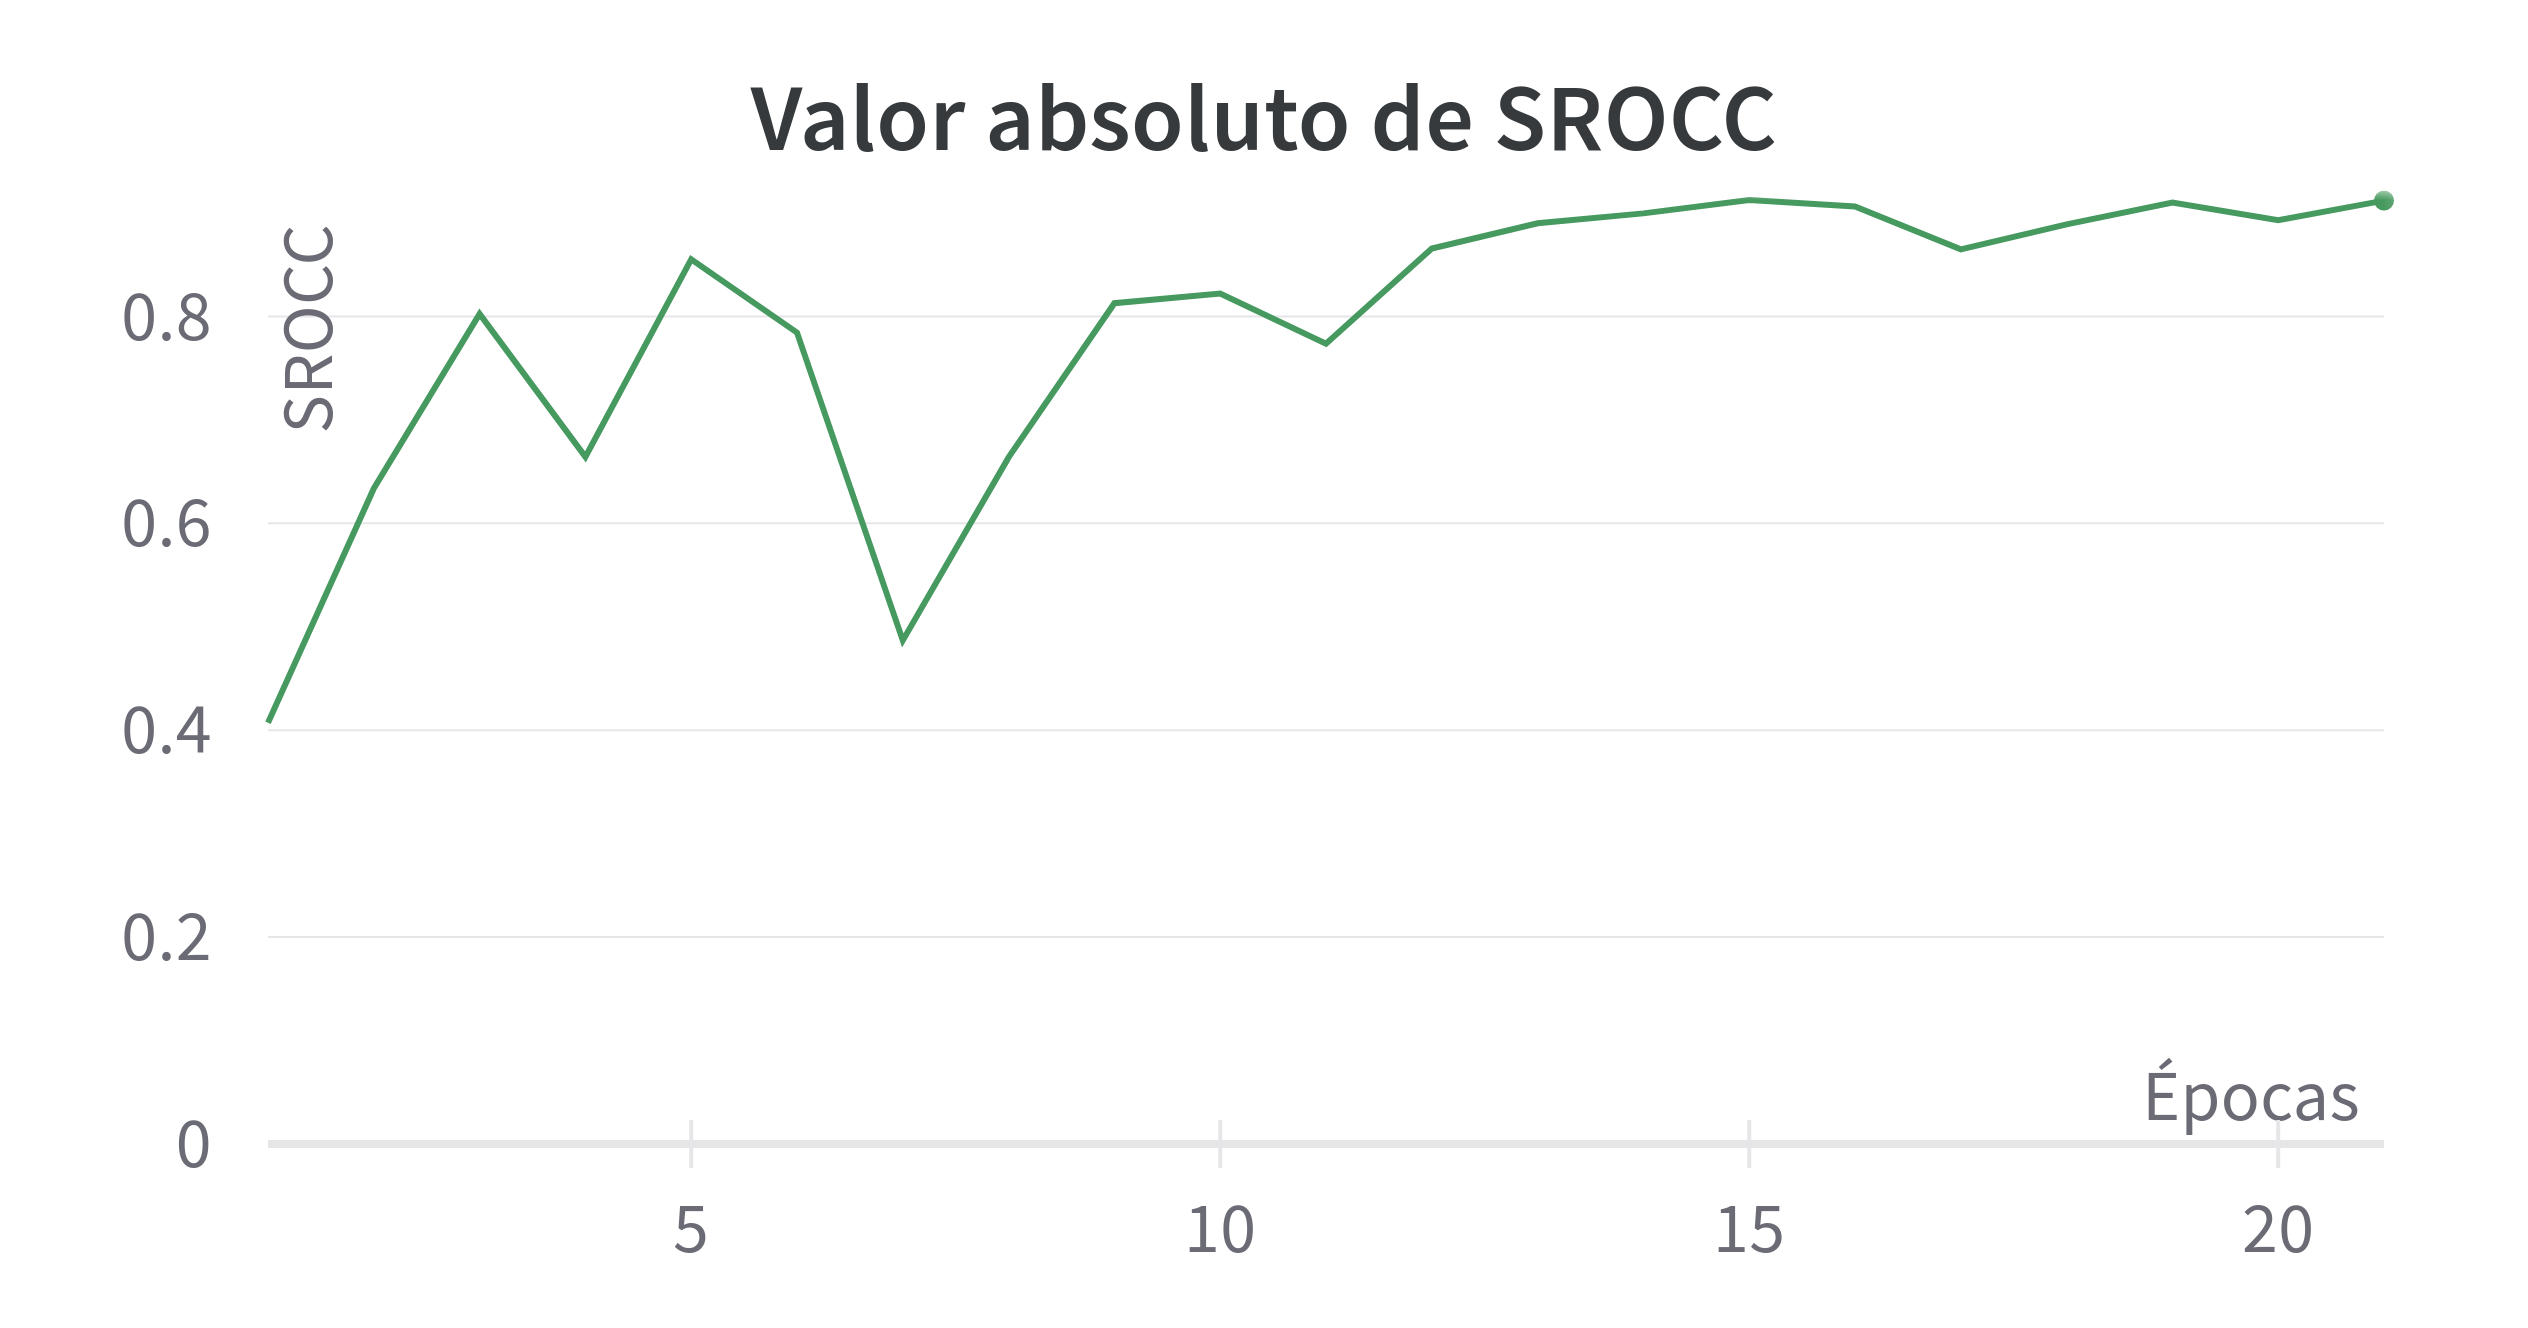
\includegraphics[width=\textwidth]{imagenes/chapter5/PreTestSROCC.png}
  \end{subfigure}
  \caption[Curvas de aprendizaje del test preliminar.]{Curvas de aprendizaje del test preliminar. 
  Cada curva describe el comportamiento medio en cada pliegue. A la derecha 
  podemos ver el comportamiento de la métrica SROCC.
} \label{fig:PreTestCurves}
\end{figure}


\subsection{Experimentos finales}
En nuestro modelo, una parte importante de la inferencia viene de la capacidad del mismo de unificar las características 
estáticas con las dinámicas. En la publicación~\cite{EnsemblePCQA} se proponen distintos métodos para la fusión
de vectores características de modelos \emph{ensemble}.
En ella, se realiza una comparativa entre cuatro métodos: la concatenación, multiplicación, convolución 1x1 y 
fusión en el dominio de fourier. 
Argumenta que cada uno de los métodos de fusión permite la interacción de los vectores 
características de distinta manera. El método de concatenación, aunque es el método 
más habitual, genera vectores de mayor dimensionalidad, hecho que puede influir 
sustancialmente al tiempo de entrenamiento e inferencia. Además, no permite una interacción directa entre los vectores. 
Es por ello que se experimenta con cada uno de estos métodos.  

La fusión por multiplicación (F1) puede provocar pérdida de información (valores cercanos a 0). 
No obstante, permiten una interacción directa de los vectores y genera un vector salida 
de menor dimensionalidad. Otro inconveniente es que tenemos normalizar, si no son 
ya iguales, a la misma dimensión los vectores. De forma similar, la fusión por convolución (F2)
permite realizar una proyección lineal de ambos vectores a uno de menor dimensionalidad. 
Por último, la fusión por \emph{bi-linear pooling} (F3) permite realizar la multiplicación de 
los vectores en el dominio de fourier, de tal forma que todos los elementos afectan al 
resultado final de forma multiplicativa, y luego proyectar 
el vector resultante a una menor dimensión utilizando algún algoritmo de proyección, 
como \emph{Count Sketch}. 

\begin{figure}[htp]
  \begin{center}
    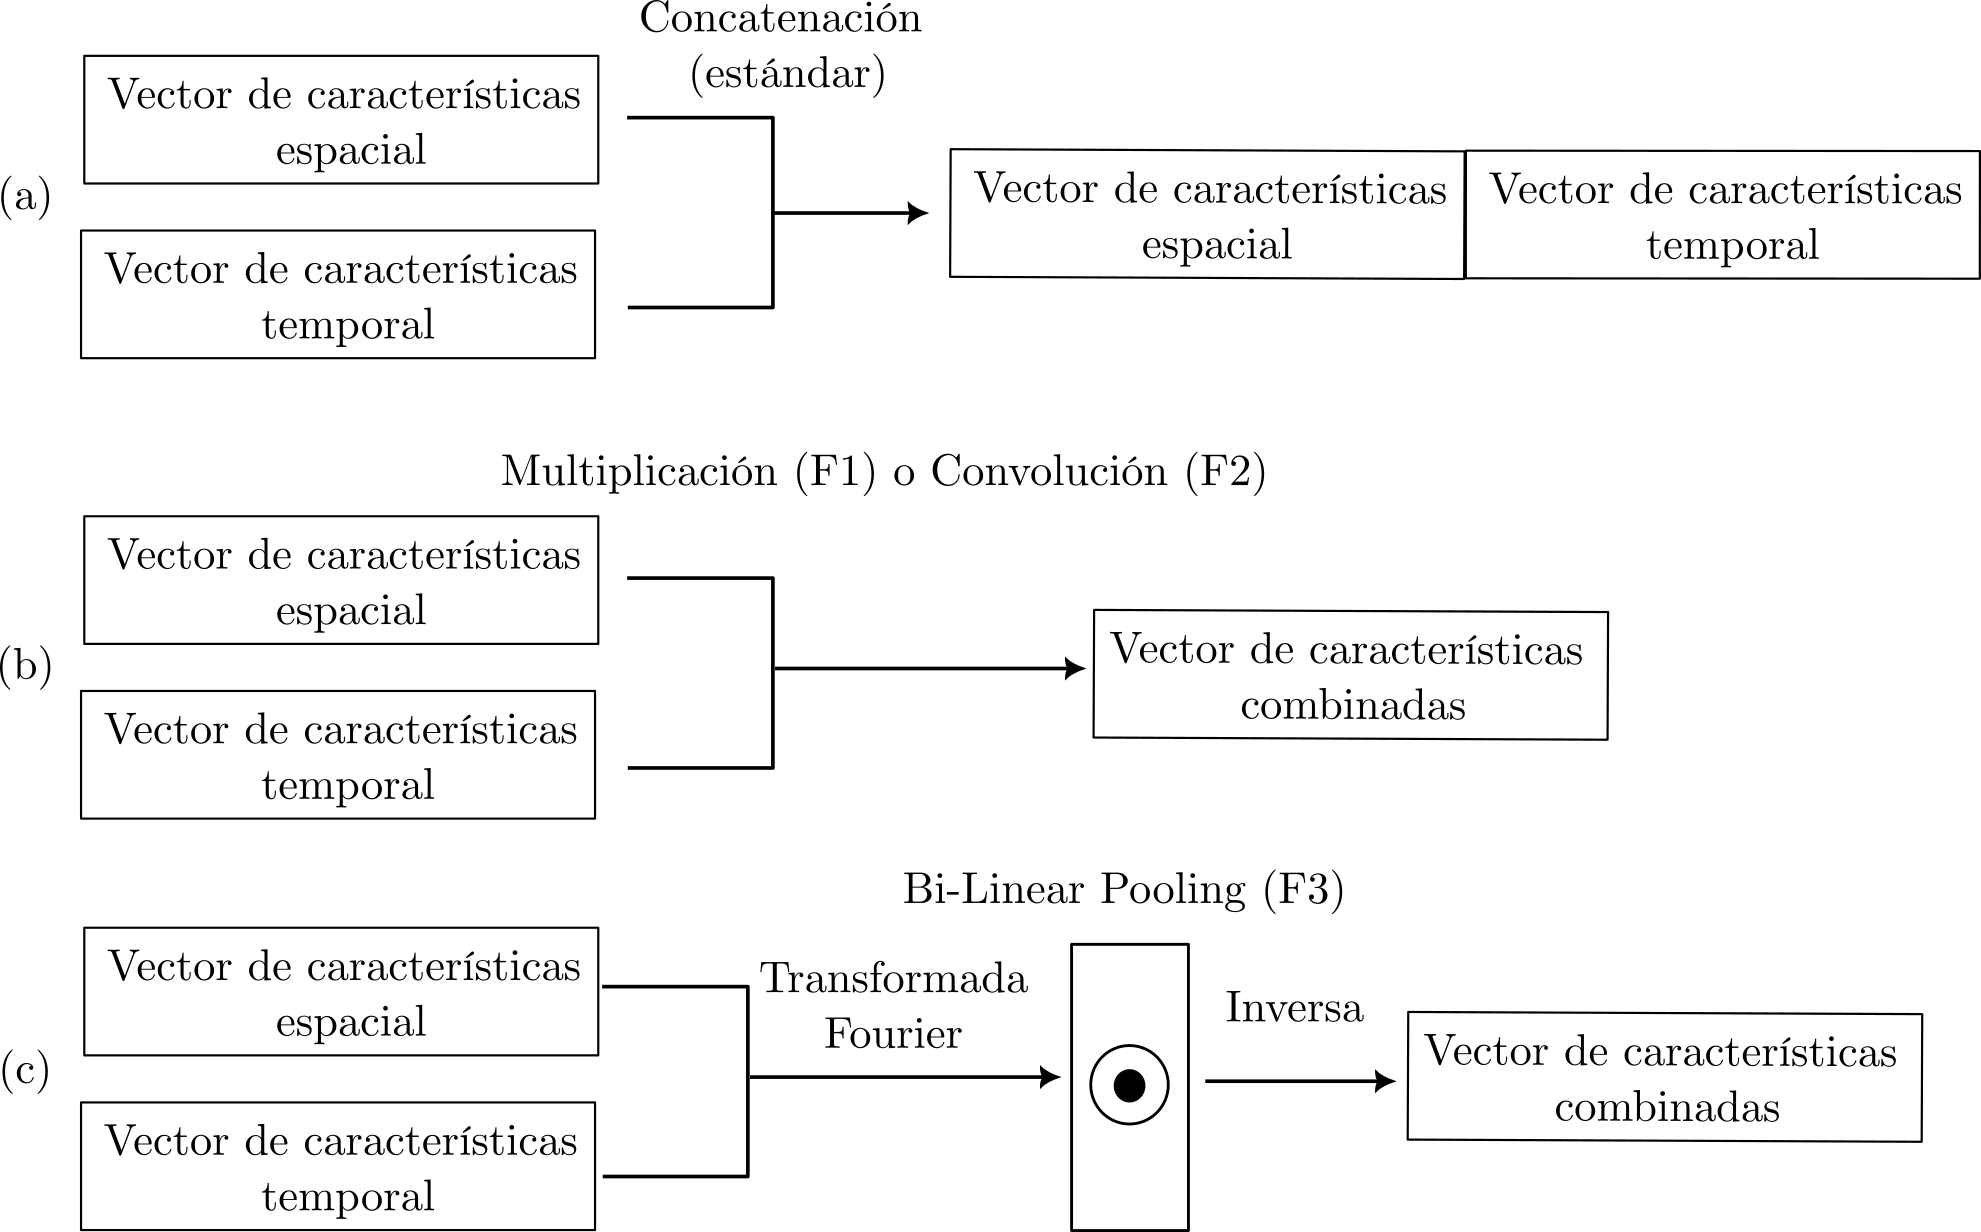
\includegraphics[width=.8\textwidth]{imagenes/chapter5/FeatureFusionExample}
  \end{center}
  \caption[Ejemplo visual de los distintos métodos de fusión a comparar.]{Ejemplo visual de los distintos métodos de fusión a comparar.
   El modelo estándar utiliza el método de concatenación (a) que genera un vector 
 característica de alta dimensionalidad. 
Por otro lado, las propuestas que figuran en (b) y (c) generan un vector de 
menor dimensionalidad, la última operando sobre el dominio de fourier.
}
  \label{fig:FeatureFusionExample}
\end{figure}

Por último, se observa que el modelo realiza un recorte aleatorio de las imágenes de entrada, 
originalmente a escala 1920x1080, durante el entrenamiento 
para ajustarlas a una escala de 224x224, lo cual reduce el tiempo de cómputo y 
evita el sobre-entrenamiento. Durante la ejecución del test, se recorta el centro de la imagen. 
Este proceso de reescalado, conocido como aumentación de datos, incrementa la cantidad de ejemplos 
y previene el sobreajuste. Sin embargo, debido a que las nubes de puntos ocupan principalmente 
la zona central de la imagen y poca proporción, se propone un reescalado uniforme a una escala de 
398x224 para obtener recortes válidos.

Para realizar la comparativa de estas mejoras, se utiliza el conjunto de datos 
médicos definidos anteriormente. Se hace la comparativa con las métricas sin 
normalizar y normalizadas a la escala 0-5, la misma con la que se entrenó VQA-PC~\cite{VQA-PC} en SJTU. 
Se entrena por 30 épocas, con el uso de \emph{early-stopping}, método utilizado para frenar el entrenamiento 
si el error de validación crece para evitar sobre-entrenamiento, con una paciencia 
de 6 épocas (en este contexto, paciencia alude a la espera de los resultados de 
las N siguientes épocas, en la que el error de validación crece, antes de terminar 
la ejecución por sobre-entrenamiento). 
Se han utilizado los mismos hiperparámetros que definido en la Tabla \ref{tab:HiperSJTU}.
Se omitirá el MSE del modelo debido a que la información principal se encuentra 
en la métrica SROCC como mencionado anteriormente al principio de la Sección \ref{sec:VQAPCSJTU}.

En la Tabla \ref{tab:SroccMedRes} hacemos 11-fold sobre nuestro conjunto de datos teniendo en cuenta las métricas originales, las métricas
normalizadas a escala 0-5 y las imágenes reescaladas. También se investiga rescalar y normalizar (última columna).
Se compara estos resultados con los demás métodos de fusión de características propuesto.
Vemos que el modelo con información previa, al utilizar el reescalado, obtiene los mejores resultados.
No obstante, F1 y F2 sin información previa consiguen acercarse a un margen de 4\% de ese valor. 
Por otro lado, la fusión F3 no logra mejorar de forma significativa. 

\begin{table}[htp]
  \scriptsize
  \centering
\begin{tabular}{|c|cccc|}
\hline
\rowcolor[HTML]{FFC702}
                       & \multicolumn{4}{c|}{\textbf{Valor medio SROCC}}                                                                                                    \\ \hline
\rowcolor[HTML]{FFC702}
\textbf{Modelo}        & \multicolumn{1}{c|}{\textbf{Estándar}} & \multicolumn{1}{c|}{\textbf{Normalizado}} & \multicolumn{1}{c|}{\textbf{Reescalado}} & \textbf{Ambos}  \\ \hline
\textbf{VQA-PC (SJTU)} & \multicolumn{1}{c|}{0.7094}            & \multicolumn{1}{c|}{\textbf{0.6235}}      & \multicolumn{1}{c|}{\textbf{0.8425}}    & 0.7126          \\ \hline
\textbf{VQA-PC F1}     & \multicolumn{1}{c|}{\textbf{0.7305}}   & \multicolumn{1}{c|}{0.6140}               & \multicolumn{1}{c|}{0.8164}             & 0.7291          \\ \hline
\textbf{VQA-PC F2}     & \multicolumn{1}{c|}{0.6816}            & \multicolumn{1}{c|}{0.5770}               & \multicolumn{1}{c|}{0.8057}             & \textbf{0.7324} \\ \hline
\textbf{VQA-PC F3}     & \multicolumn{1}{c|}{0.7080}            & \multicolumn{1}{c|}{0.5671}      & \multicolumn{1}{c|}{0.7482}             & 0.7006          \\ \hline
\end{tabular}
\caption[Valor medio sobre imágenes médicas.]{Tabla de resultados iniciales sobre imágenes médicas. 
Partimos del modelo pre-entrenado de la publicación original~\cite{VQA-PC} sobre SJTU y 
a continuación desde 0 con los métodos de fusión de característica.
}
\label{tab:SroccMedRes}
\end{table}

Los resultados son prometedores. El modelo con información adicional sobre otros 
tipos de distorsiones, conocimiento del conjunto SJTU, es el que obtiene el mejor 
resultado tras reescalar las imágenes, seguido por el modelo entrenado desde 0 
con la fusión por multiplicación (F1). No obstante, se ha observado cierta 
variabilidad en los resultados de cada pliegue, como se observa en la Tabla \ref{tab:STDevMed}.
Esto puede ser debido a diversos factores, desde la dificultad del modelo de 
aprender las características relevantes en tan pocas épocas, por la falta 
de ejemplos en este pequeño conjunto de imágenes médicas, por la variabilidad 
entre nubes de puntos (pocos ejemplos similares y muchas partes del cuerpo) 
o por dificultades en la generación de etiquetas sintéticas de calidad. 
Además, observándose detenidamente los valores obtenidos en cada pliegue, 
se observa una alta variabilidad para un ejemplo en concreto, el último pliegue, 
con SROCC a más de 3 desviaciones típicas para los casos F1-F3.  Es por ello, 
que se puede observar la mediana de cada modelo en la Tabla \ref{tab:PercentileMed}.

Para validar el rápido aprendizaje de los métodos F1-F3 y la posible mejora 
sobre el método de concatenación, se experimenta utilizar el modelo VQA-PC sin 
modificaciones desde 0 sobre las imágenes reescaladas (véase Tabla \ref{tab:VQAF0}).
Se obtiene en media resultados algo peor que el modelo 
pre-entrenado, remarcando la importancia de información adicional y etapas 
de entrenamiento más largas a la hora de lidiar con algunas nubes de puntos, aunque su
mediana es la mejor de los 4 modelos sin pre-entrenar en distorsiones. 
Se determina que, para un conjunto de datos pequeños, las mejoras F1-F3 no son significativas sin información adicional. 
Dado la importancia de la información adicional sobre las distorsiones a la 
hora de estimar la calidad de las imágenes de nuestro pequeño conjunto médico, 
se propone pre-entrenar sobre el conjunto LS-SJTU-PCQA.
En este caso, se utilizará las imaǵenes reescaladas y las métricas sin normalizar, 
dado que se ha observado anteriormente que es la mejor combinación. Sobre los 
datos de LS-SJTU-PCQA, se invierte el MOS para que pase a representar el nivel 
de distorsión en lugar del nivel de calidad en escala 0-1, para que se asemeje a los 
valores sintéticos sin normalizar, y también utilizamos imágenes reescaladas.

Se observa una mejora significativa en los métodos F2-F3, y se logra 
pasar la barrera del 90\% en la mediana de los métodos F0-F2 (véase Tabla \ref{tab:LS-SJTU-FN}).
Gracias a la información adicional hemos logrado valores mucho mejores, llegando a 
obtener una correlación del 88\% de media, con mediana al 94\%, utilizando el modelo F2. 
En general, poseer información adicional ha resultado ser crucial para el aprendijaze 
del modelo. No obstante, la distribución de esa información es de suma importancia a la 
hora de determinar la capacidad de generalización del modelo. Vemos que con el nuevo 
conjunto de datos, el modelo F0 recibe un incremento en desviación típica al
volverse incapaz de predecir correctamente el último pliegue al igual que los demás métodos.  

\begin{table}[htp]
  \scriptsize
  \centering
\begin{tabular}{|c|cccc|}
\hline
\rowcolor[HTML]{FFC702}
                       & \multicolumn{4}{c|}{\textbf{Desviación típica SROCC}}                                                                                                \\ \hline
\rowcolor[HTML]{FFC702}
\textbf{Modelo}        & \multicolumn{1}{c|}{\textbf{Estándar}} & \multicolumn{1}{c|}{\textbf{Normalizado}} & \multicolumn{1}{c|}{\textbf{Reescalado}} & \textbf{Ambos}  \\ \hline
\textbf{VQA-PC (SJTU)} & \multicolumn{1}{c|}{0.1448}            & \multicolumn{1}{c|}{0.2357}               & \multicolumn{1}{c|}{\textbf{0.0668}}    & 0.1335          \\ \hline
\textbf{VQA-PC F1}     & \multicolumn{1}{c|}{\textbf{0.1222}}   & \multicolumn{1}{c|}{0.1402}               & \multicolumn{1}{c|}{0.1752}             & 0.2250          \\ \hline
\textbf{VQA-PC F2}     & \multicolumn{1}{c|}{0.1462}            & \multicolumn{1}{c|}{0.1905}               & \multicolumn{1}{c|}{0.1741}             & \textbf{0.1187} \\ \hline
\textbf{VQA-PC F3}     & \multicolumn{1}{c|}{0.1507}            & \multicolumn{1}{c|}{\textbf{0.1304}}      & \multicolumn{1}{c|}{0.1326}             & 0.1462          \\ \hline
\end{tabular}
\caption[Desviación típica de los resultados médicos]{Desviación típica de los 
resultados obtenidos. Se observa que la mejora del reescalado de las imágenes 
de entrada mejora la estabilidad del modelo inicial. El método de fusión F3 
es el más estable en todos los casos. }
\label{tab:STDevMed}
\end{table}

\begin{table}[htp]
  \scriptsize
  \centering
\begin{tabular}{|c|cccc|}
\hline
\rowcolor[HTML]{FFC702}
                       & \multicolumn{4}{c|}{\textbf{Mediana SROCC}}                                                                                                          \\ \hline
\rowcolor[HTML]{FFC702}
\textbf{Modelo}        & \multicolumn{1}{c|}{\textbf{Estándar}} & \multicolumn{1}{c|}{\textbf{Normalizado}} & \multicolumn{1}{c|}{\textbf{Reescalado}} & \textbf{Ambos}  \\ \hline
\textbf{VQA-PC (SJTU)} & \multicolumn{1}{c|}{\textbf{0.7400}}   & \multicolumn{1}{c|}{\textbf{0.7510}}      & \multicolumn{1}{c|}{0.8417}             & 0.7434          \\ \hline
\textbf{VQA-PC F1}     & \multicolumn{1}{c|}{0.7022}            & \multicolumn{1}{c|}{0.6331}               & \multicolumn{1}{c|}{\textbf{0.8636}}    & \textbf{0.7849} \\ \hline
\textbf{VQA-PC F2}     & \multicolumn{1}{c|}{0.6350}            & \multicolumn{1}{c|}{0.5955}               & \multicolumn{1}{c|}{0.8538}             & 0.7165          \\ \hline
\textbf{VQA-PC F3}     & \multicolumn{1}{c|}{0.7118}            & \multicolumn{1}{c|}{0.5179}               & \multicolumn{1}{c|}{0.7518}             & 0.7334          \\ \hline
\end{tabular}
\caption[Mediana de los valores sobre imágenes médicas.]{
  Mediana de los valores obtenidos. Se observa una mejora significativa para 
  los métodos F1 y F2. También es evidente la estabilidad del modelo pre-entrenado
  sobre SJTU. 
}
\label{tab:PercentileMed}
\end{table}


\begin{table}[htp] 
  \scriptsize
  \centering
  \begin{tabular}{|c|c|c|c|}
\hline
\rowcolor[HTML]{FFC702}
                       & \multicolumn{3}{c|}{\textbf{SROCC}}                                                                                                          \\ \hline
\rowcolor[HTML]{FFC702}
\textbf{Modelo}        & \multicolumn{1}{c|}{\textbf{Media}} & \multicolumn{1}{c|}{\textbf{Desviación}} & \multicolumn{1}{c|}{\textbf{Mediana}} \\ \hline
\textbf{VQA-PC F0} & \multicolumn{1}{c|}{\textbf{0.8261}}   & \multicolumn{1}{c|}{0.1589}      & \multicolumn{1}{c|}{\textbf{0.8657}}      \\ \hline
  \end{tabular}
  \caption[Resultados del método original sin pre-entrenar sobre imágenes reescaladas.]{
    Resultados del método original con modelo original sin pre-entrenar sobre imágenes médicas reescaladas. 
  
}
\label{tab:VQAF0}
\end{table}

\begin{table}[H]
  \scriptsize 
  \centering
\begin{tabular}{|c|c|c|c|}
\hline
\rowcolor[HTML]{FFC702}
                       & \multicolumn{3}{c|}{\textbf{SROCC}}                                                                                                          \\ \hline
\rowcolor[HTML]{FFC702}
\textbf{Modelo}    & \textbf{Media} & \textbf{Desviación} & \textbf{Mediana} \\ \hline
\textbf{VQA-PC F0} & 0.8325           & 0.2017              & 0.9140           \\ \hline
\textbf{VQA-PC F1} & 0.8242           & 0.2025              & 0.9095           \\ \hline
\textbf{VQA-PC F2} & \textbf{0.8757}  & \textbf{0.1468}     & \textbf{0.9347}  \\ \hline
\textbf{VQA-PC F3} & 0.8071           & 0.1811              & 0.8692           \\ \hline
\end{tabular}
\caption[Resultados en imágenes médicas reescaladas entrenando en LS-SJTU-PCQA.]{
  Resultados en imágenes médicas reescaladas con modelos pre-entrenados 
  sobre el conjunto de datos LS-SJTU-PCQA. 
}\label{tab:LS-SJTU-FN}
\end{table}
